\documentclass[a4paper, 12pt]{article}
\usepackage{geometry}
\geometry{verbose,a4paper,tmargin=2cm,bmargin=2cm,lmargin=2cm,rmargin=2cm}
\usepackage{fontspec}
\setmainfont[
  Ligatures=TeX,
  Extension=.otf,
  UprightFont=*-regular,
  ItalicFont=*-italic,
  BoldFont=*-bold,
  BoldItalicFont=*-bolditalic,
]{xits}
\usepackage[english,russian]{babel}

\newif\ifisinsp
\newif\ifisone
\newif\ifisname
\newif\ifisnum
\isinsptrue
\isonetrue
\isnamefalse
\isnumtrue

\def \labtype {Лабораторная}
% Это для нумерации страниц после титульника
\usepackage{fancyhdr}
\pagestyle{fancy}
\renewcommand{\headrulewidth}{0pt}
\fancyfoot[C] {\thepage}

\def \labtype {Домашняя}
\def \labnum {1}
\def \labsubj {Сети ЭВМ и телекоммуникации}
\def \labauthor {Чебыкин И. Б.}
\def \labgroup {P3301}
\def \labinsp {Шинкарук Д. Н.}
\isnamefalse

\usepackage{graphicx,tabularx}

\usepackage{caption}

\captionsetup{labelsep=period}
\pagestyle{fancy}
\begin{document}
\begin{titlepage}
	\begin{center}
		\large
		Университет ИТМО

		\vspace{0.25cm}
		
		Факультет программной инженерии и компьютерной техники
		
		Кафедра вычислительной техники
		\vfill
		
		\textsc{\labtype\spaceработа \ifisnum № \labnum{} \fi по дисциплине \\"\labsubj" \ifisname\small \\ \labname \fi}
			
		\bigskip
	\end{center}
	\vfill
	\vfill
	
	\begin{flushright}
	\ifisone
	Выполнил: \labauthor
	\else
	Выполнили: \labauthor
	\fi

	\vspace{0.25cm}
	Группа: \labgroup
			
	\vspace{0.25cm}
	\ifisinsp
	Проверяющий: \labinsp
	\fi
	\end{flushright}
	\vfill
	
	\begin{center}
	СПб, \the\year
	\end{center}
\end{titlepage}


\section{Описание работы}
Цель работы: изучение методов логического и физического кодирования,
используемых в цифровых сетях передачи данных.
В процессе выполнения домашнего задания необходимо выполнить
логическое и физическое кодирование исходного сообщения в соответствии с
заданными методами кодирования, провести сравнительный анализ
рассматриваемых методов кодирования, выбрать и обосновать наилучший метод
для передачи исходного сообщения.
\section{Порядок выполнения задания}
\begin{enumerate}
\item Сформировать исходное сообщение.
\item Выполнить физическое кодирование исходного сообщения не менее, чем
тремя способами, включая, в качестве обязательного, манчестерское кодированиe.
\item Выполнить логическое кодирование исходного сообщения, используя
избыточное кодирование 4В/5В и скремблирование.
\item Выполнить сравнительный анализ рассмотренных способов
кодирования и выбрать наилучший способ для передачи исходного сообщения.
\end{enumerate}
\newpage
\section{Физическое кодирование}
\subsection{Исходное сообщение}
Данные: Чебыкин И.Б.

в шестнадцатеричном коде: \verb|D7 E5 E1 FB EA E8 ED 20 C8 2E C1 2E|

в двоичном коде:

\begin{verbatim}
	11010111 11100101 11100001 11111011 11101010 11101000
	11101101 00100000 11001000 00101110 11000001
\end{verbatim}

длина сообщения: 12 байт (96 бит)
\subsection{NRZ}

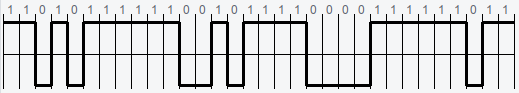
\includegraphics[scale=0.7]{img/nrz_norm.png}

$f_0 = \frac{1}{2t_b} = 5$ МГц

$f_H = \frac{1}{12t_b} = 0,833$ МГц

$f_B = f_0 \cdot 7 = 35$ МГц

$F = f_B - f_H = 34,167$ МГц

$F_{cp} = 1,875$ МГц

\subsection{RZ}
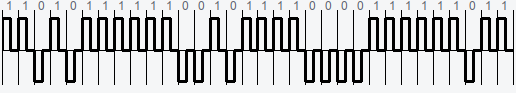
\includegraphics[scale=0.7]{img/rz_norm.png}

$f_0 = \frac{1}{t_b} = 10$ МГц

$f_H = \frac{1}{2t_b} = 5$ МГц

$f_B = f_0 \cdot 7 = 70$ МГц

$F = f_B - f_H = 65$ МГц

$F_{cp} = 8,125$ МГц
\subsection{Mанчестерский}
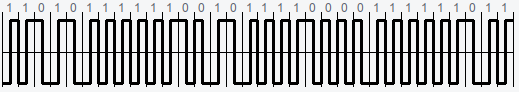
\includegraphics[scale=0.7]{img/m_norm.png}

$f_0 = \frac{1}{t_b} = 10$ МГц

$f_H = \frac{1}{2t_b} = 5$ МГц

$f_B = f_0 \cdot 7 = 70$ МГц

$F = f_B - f_H = 65$ МГц

$F_{cp} = 8,125$ МГц
\subsection{Результаты сравнительного анализа}
\begin{table}[!h]
\begin{tabular}{|c|c|c|c|c|c|}
\hline
    & $f_0$ & $f_H$, МГц & $f_B$, МГц & $F$, МГц & $F_{cp}$, МГц \\ \hline
NRZ & 5     & 0,833      & 35         & 34,167   & 1,875         \\ \hline
RZ  & 10    & 5          & 70         & 65       & 8,125         \\ \hline
M   & 10    & 5          & 70         & 65       & 8,125         \\ \hline
\end{tabular}
\end{table}

\begin{table}[!h]
\begin{tabular}{|c|c|c|c|c|c|}
\hline
                                    & NRZ & RZ & M \\ \hline
Минимизация спектра                 & +   & -  & - \\ \hline
Самосинхронизация                   & -   & +  & + \\ \hline
Постоянная составляющая             & +   & -  & - \\ \hline
Обнаружение ошибок и их исправление & -   & +  & + \\ \hline
Низкая стоимость реализации         & +   & -  & + \\ \hline
\end{tabular}
\end{table}

Исходя из полученных результатов можно выбрать следующие способы кодирования:

RZ -- хоть он и дороже, чем NRZ и манчестерский, свойство самосинхронизации
позволяет не вести отдельную линию для синхронизации сигнала.

Манчестерский -- т.к. имеет невысокую стоимость реализации.

\section{Логического кодирование}
\subsection{Исходное сообщение}
в шестнадцатеричном коде: \verb|DB F8 BE 27 B7 E5 B9 2E 6E 9E D4 A9 CD 26 9C|

в двоичном коде:

\begin{verbatim}
 11011011 11111000 10111110 00100111 10110111 11100101 10111001 00101110
 01101110 10011110 11010100 10101001 11001101 00100110 10011100
\end{verbatim}

длина сообщения: 15 байт (120 бит)
избыточность: $3/12 = 0,25 = 25\%$

\subsection{RZ}
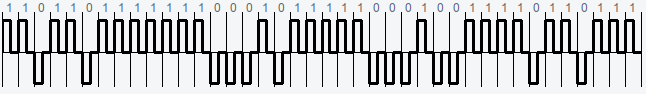
\includegraphics[scale=0.7]{img/rz_redu.png}

$f_0 = \frac{1}{t_b} = 10$ МГц

$f_H = \frac{1}{2t_b} = 5$ МГц

$f_B = f_0 \cdot 7 = 70$ МГц

$F = f_B - f_H = 65$ МГц

$F_{cp} = 8$ МГц
\subsection{Mанчестерский}
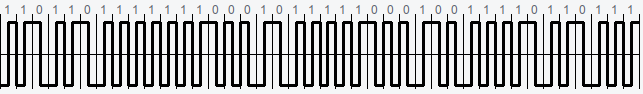
\includegraphics[scale=0.7]{img/m_redu.png}

$f_0 = \frac{1}{t_b} = 10$ МГц

$f_H = \frac{1}{2t_b} = 5$ МГц

$f_B = f_0 \cdot 7 = 70$ МГц

$F = f_B - f_H = 65$ МГц

$F_{cp} = 8$ МГц
\subsection{Результаты сравнительного анализа}
\begin{table}[!h]
\begin{tabular}{|c|c|c|c|c|c|}
\hline
    & $f_0$ & $f_H$, МГц & $f_B$, МГц & $F$, МГц & $F_{cp}$, МГц \\ \hline
RZ  & 10    & 5          & 70         & 65       & 8             \\ \hline
M   & 10    & 5          & 70         & 65       & 8             \\ \hline
\end{tabular}
\end{table}

Исходя из сравнения видно, что эти методы идентичны, поэтому выгоднее
выбрать манчестерский способ из-за низкой стоимости реализации.
\subsection{Скремблирование}
Т.к. мы кодируем не более 32 битов, то достаточно выбрать полином $B_i = A_i \oplus B_i-3 \oplus B_i-5$
в шестнадцатеричном коде: \verb|C8 B6 85 7F E8 BA 70 B3 37 7A 58 F7|

в двоичном коде:

\begin{verbatim}
 11001000 10110110 10000101 01111111 11101000 10111010
 01110000 10110011 00110111 01111010 01011000 11110111
\end{verbatim}
\begin{table}[!h]
\scriptsize
\begin{tabular}{|l|l|l|l|}
\hline
B1 = А1 = 1          &В9 = А9 ⊕ В6 ⊕ В4 = 1    &В17 = А17 ⊕ В14 ⊕ В12 = 1&В25 = А25 ⊕ В22 ⊕ В20 = 0 \\ \hline
В2 = А2 = 1          &В10 = А10 ⊕ В7 ⊕ В5 = 0  &В18 = А18 ⊕ В15 ⊕ В13 = 0&В26 = А26 ⊕ В23 ⊕ В21 = 1 \\ \hline
В3 = А3 = 0          &В11 = А11 ⊕ В8 ⊕ В6 = 1  &В19 = А19 ⊕ В16 ⊕ В14 = 0&В27 = А27 ⊕ В24 ⊕ В22 = 1 \\ \hline
В4 = А4 ⊕ В1 = 0     &В12 = А12 ⊕ В9 ⊕ В7 = 1  &В20 = А20 ⊕ В17 ⊕ В15 = 0&В28 = А28 ⊕ В25 ⊕ В23 = 1 \\ \hline
В5 = А5 ⊕ В2 = 1     &В13 = А13 ⊕ В10 ⊕ В8 = 0 &В21 = А21 ⊕ В18 ⊕ В16 = 0&В29 = А29 ⊕ В26 ⊕ В24 = 1 \\ \hline
В6 = А6 ⊕ В3 ⊕ В1 = 0&В14 = А14 ⊕ В11 ⊕ В9 = 1 &В22 = А22 ⊕ В19 ⊕ В17 = 1&В30 = А30 ⊕ В27 ⊕ В25 = 1 \\ \hline
В7 = А7 ⊕ В4 ⊕ В2 = 0&В15 = А15 ⊕ В12 ⊕ В10 = 1&В23 = А23 ⊕ В20 ⊕ В18 = 0&В31 = А31 ⊕ В28 ⊕ В26 = 1 \\ \hline
В8 = А8 ⊕ В5 ⊕ В3 = 0&В16 = А16 ⊕ В13 ⊕ В11 = 0&В24 = А24 ⊕ В21 ⊕ В19 = 1&В32 = А32 ⊕ В29 ⊕ В27 = 1 \\ \hline
\end{tabular}
\end{table}
\subsection{RZ}
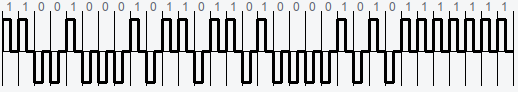
\includegraphics[scale=0.7]{img/rz_scra.png}

$f_0 = \frac{1}{t_b} = 10$ МГц

$f_H = \frac{1}{2t_b} = 5$ МГц

$f_B = f_0 \cdot 7 = 70$ МГц

$F = f_B - f_H = 65$ МГц

$F_{cp} = 7,5$ МГц
\subsection{Mанчестерский}
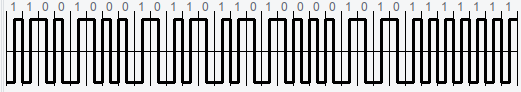
\includegraphics[scale=0.7]{img/m_scra.png}

$f_0 = \frac{1}{t_b} = 10$ МГц

$f_H = \frac{1}{2t_b} = 5$ МГц

$f_B = f_0 \cdot 7 = 70$ МГц

$F = f_B - f_H = 65$ МГц

$F_{cp} = 7,5$ МГц
\subsection{Результаты сравнительного анализа}

\begin{table}[!h]
\begin{tabular}{|c|c|c|c|c|c|}
\hline
    & $f_0$ & $f_H$, МГц & $f_B$, МГц & $F$, МГц & $F_{cp}$, МГц \\ \hline
RZ  & 10    & 5          & 70         & 65       & 7,5           \\ \hline
M   & 10    & 5          & 70         & 65       & 7,5           \\ \hline
\end{tabular}
\end{table}
Опять же видно, что эти методы идентичны, поэтому выгоднее
выбрать манчестерский способ из-за низкой стоимости реализации.
\section{Вывод}
\end{document}
